Octrees are a foundational data structure for fast algorithms in $\mathbb{R}^3$. Writing software for octrees that can be distributed across parallel computing systems is challenging, demonstrated by the limited availability of open-source software \cite{BursteddeWilcoxGhattas11,fernando2020github}. This is inspite of their ubiquity in scientific computing applications from adaptive finite-element methods to many-body algorithms \cite{sundar2008bottom}. We present Rusty Tree, an implementation of MPI-distributed octrees with a complete Python interface. Rusty Tree is a proof of concept for Rust as a tool for high-performance computational science. We document our experience in developing Rusty Tree, and use it as a tool to explore the current landscape of scientific computing with Rust. From multithreading, and developing a Python interface, to distributing applications with MPI, writing Rusty Tree involved using much of Rust's scientific computing ecosystem. 

\subsection*{Parallel Octrees}

As mentioned in section \ref{sec:2_2}, there are multiple representations of octrees. We choose a linear octree representation, in which we discard interior nodes and store a list of leaves, as in our previous work PyExaFMM \cite{kailasa2022pyexafmm}. These lie in contrast to pointer based octrees in which each node stores pointers to its parent as well as children, which have a relatively higher storage cost, in addition to a synchronisation and communication overhead for parallel implementations that must keep track of pointers across nodes \cite{tu2005scalable}. 

Pointer based octrees are usually constructed `top down'. A user specifies a threshold for the maximum number of particles in a leaf node, $n_{\text{crit}}$, and a unit cube encapsulating the problem domain is refined until this is satisfied. After refinement, one can optionally `balance' adjacent leaf nodes such that adjacent nodes obey a relative size constraint. However, translating this logic to a parallel setting is challenging. Constructing octrees `top down' involve significant data communication. As the point distribution on each processor isn't known a priori, each processor is responsible for constructing its own octree from a random batch of points, reconciling the trees across nodes then requiring a global parallel merge. Furthermore, there are likely to be significant overlaps and duplicates in the nodes of each processor's octree, which would result further refinement after the parallel merge in order to satisfy the $n_{\text{crit}}$ constraint. Balancing the octree, as well as load-balancing the work assigned to each processor, must be done as post-processing steps.

For these reasons, Sundar et al introduced `bottom up' tree construction \cite{sundar2008bottom}. `Bottom up' refers to the fact that octrees are constructed from the leaf level upwards, which allows us to incorporate the initial data distribution into our algorithms. In order to do this they use a space-filling curve that passes through each octant, for which they choose a Morton encoding.

Given a set of distributed point data spread across $n_p$ processors, our strategy is as follows:

\begin{enumerate}
    \item Generate a Morton key for each point at the leaf level corresponding to a user defined octree depth.
    \item Perform a parallel sort of these leaf octants using MPI, such that processors with adjacent MPI ranks have adjacent data.
    \item \textit{Linearise} leaves on each processor, such that their leaves do not overlap, in a manner that favours smaller leaves over larger ones, as in algorithm (\ref{alg:sec_2_4:linearise_octree}). 
    \item \textit{Complete} the space defined by the leaves on each processor, and find the domain occupied by their leaves, see figure (\ref{fig:sec_2_4:complete}) and algorithm (\ref{alg:sec_2_4:complete_region}). Define the coarsest nodes of this set as \textit{seeds}.
    \item Construct a \textit{block tree}, by completing the space between the seeds with the minimum spanning set of nodes, described in algorithm (\ref{alg:sec_2_4:complete_octree}). The nodes of this block tree are referred to as \textit{blocks}. This gives us a distributed coarse complete linear octree that is based on the underlying data distribution.
    \item Point data is communicated to the processor containing its associated block, and the blocks are refined based on $n_{\text{crit}}$, providing the final linear octree tree.
    \item Optionally, the tree is \textit{balanced}. This can be done for the local subtree on each processor using algorithm (\ref{alg:sec_2_4:balance_octree}). The locally balanced trees can then be sorted in parallel again, and locally linearized as in step (3), to provide a globally balanced tree.
\end{enumerate}

This approach is summarised in algorithm (\ref{alg:sec_2_4:point2octree}). The complexity of this process is bounded by the parallel sorts, which for randomly distributed point data, run in $O(N_{\text{leaf}} \log (N_{\text{leaf}}))$ work and $O(\frac{N_{\text{leaf}}}{n_p} \log(\frac{N_{\text{leaf}}}{n_p}) + n_p \log (n_p))$ time where $N_{\text{leaf}}$ is the number of leaves in the final octree, and $n_p$ is the number of processors (see appendix \ref{app:a_2_complexity_tree_construction} for a derivation). This makes the efficiency of the parallel sort a bottleneck in tree construction.

\begin{figure}
    \centerline{
\includegraphics[width=\linewidth]{ch_2/morton.pdf}}
    \caption{How to Morton encode a node in an octree. The node is described by an `anchor' coordinate.}
    \label{fig:sec_2_4:morton}
\end{figure}

\begin{algorithm}
    \caption{\textbf{Construct Distributed Octree (Parallel)}}
    \label{alg:sec_2_4:point2octree}
    \begin{algorithmic}
        \STATE \textbf{Input}: A distributed list of points $L$, and a parameter $n_{crit}$ specifying the maximum number of points per octant.
        \STATE \textbf{Output}: A complete linear octree, $B$. 
        \STATE \textbf{Work}: $O(n \log n)$, where $n$=len($L$).
        \STATE \textbf{Storage}: $O(n)$, where $n$=len($L$).
        
        \STATE $F \gets $ [Octant($p$, MaxDepth), $\forall p \in L$]
        \STATE ParallelSort(F)
        \STATE $B \gets $ BlockPartition($F$), using algorithm (\ref{alg:sec_2_4:block_partition})
        \FOR {$b \in B$}
            \IF {NumberOfPoints($b$) $>$ $n_{crit}$}
                \STATE $B \gets B - b + $ Children($b$)
            \ENDIF
        \ENDFOR

        \STATE \\\# Optional Balancing over subtrees, $f$.

        \IF {Balance = True}
            \FOR {$f \in F$}
                \STATE Balance($f$), using algorithm (\ref{alg:sec_2_4:balance_octree})
            \ENDFOR

            \STATE ParallelSort($F$)
            
            \FOR {$f \in F$}
                \STATE Linearise($f$), using algorithm (\ref{alg:sec_2_4:linearise_octree})
            \ENDFOR
        \ENDIF

    \end{algorithmic}
\end{algorithm}

\begin{figure}
    \centerline{
\includegraphics[width=0.9\linewidth]{ch_2/complete_region.pdf}}
    \caption{Adapted from \cite{sundar2008bottom}, describing the algorithms in $\mathbb{R}^2$ for clarity. Figure (b) shows the minimal tree constructed using algorithm (\ref{alg:sec_2_4:complete_region}) where the two octants in (a) are used as an input. Figure (c) shows a selection of \textit{seeds}, which are used as an input to algorithm (\ref{alg:sec_2_4:complete_octree}), resulting in (d). Figure (d) also shows two octants generated to complete the domain.  The first one is the coarsest ancestor of the least input octant which does not overlap with the least octant in the input. The second is the coarsest ancestor of the greatest possible octant, which doesn't overlap with it.}
    \label{fig:sec_2_4:complete}
\end{figure}

We extend the approach first presented by Sundar et al in two key ways. Firstly, we use HykSort \cite{sundar2013hyksort}, a variant of parallel hypercube sort, which reduces global data communication cost in comparison to a parallel sample sort based on \pythoninline{MPIAllToAllv}. We cover the relative merits of HykSort in the next subsection. Secondly, balancing algorithms in the original implementation are based on a `ripple propagation scheme'. The `ripple effect' is the phenomenon that describes how octants can effect immediately adjacent octants if they are split, or combined, which can trigger further changes, that must then be propagated across the network. These algorithms involve relatively complex communication schemes in their implementation. We therefore replace this with an algorithm which, starting with an unbalanced tree, finds the locally balanced tree on each processor using algorithm (\ref{alg:sec_2_4:balance_octree}), performs another parallel sort using HykSort, and removes overlaps, favouring smaller octants, using algorithm (\ref{alg:sec_2_4:linearise_octree}). This guarantees that the balance condition is maintained. This logic will recover a globally balanced tree, with a significantly simpler communication pattern. This strategy has been previously been implemented in large scale parallel octree construction \cite{malhotra2015pvfmm}, and has been shown to obtain similar runtimes to calculate balancing when compared to ripple propagation based schemes \cite{suh2020evaluation}.

Load balancing across processors, while maintaining Morton order is challenging. Currently, the data partitioning imposed by the parallel sort imposes a degree of load balancing, which we examine for different geometries in figure (\ref{fig:sec_2_4:tree_comparison}c). However, in future we would like to extend our work to incorporate an explicit load balancing step. Our current idea is based on a sample sort, with splitter selection and bucket sizes chosen to reflect the mean load we wish to assign to each processor.

\begin{figure}
    \centerline{
\includegraphics[width=\linewidth]{ch_2/rayon.pdf}}
    \caption{Optimising Morton encodings using shared memory parallelism and lookup tables.}
    \label{fig:sec_2_4:rayon}
\end{figure}

\begin{algorithm}
    \caption{\textbf{Morton Order (Sequential)}: Find the lesser of wo Morton keys with different anchors.}
    \label{alg:sec_2_4:morton_ordering}
    \begin{algorithmic}
    
        \STATE \textbf{Input}: Two Morton ids, $A$ and $B$, with different anchors.
        \STATE \textbf{Output}: $R$, the lesser Morton key.
        
        \STATE $X_i \gets (A_i \bigoplus B_i)$, $i \in {x, y, z}$
        \STATE $e \gets \arg \max \left ( \left \lfloor \log_2(X_i) \right \rfloor \right )$
        \IF { $A_e < B_e$ }
            \STATE $R \gets A$
        \ELSE
            \STATE $R \gets B$
        \ENDIF
    \end{algorithmic}
\end{algorithm}
    

\begin{algorithm}
    \caption{\textbf{Remove Overlaps From Sorted List of Octants (Sequential)} - \texttt{Linearise}. Favour smaller octants over larger overlapping octants.}
    \label{alg:sec_2_4:linearise_octree}
    \begin{algorithmic}
    
        \STATE \textbf{Input}: A sorted list of octants, $W$.
        \STATE \textbf{Output}: $R$, an octree with no overlaps.
        \STATE \textbf{Work}: $O(n)$, where $n$=len($W$).
        \STATE \textbf{Storage}: $O(n)$, where $n$=len($W$).
    
        \FOR{i $\gets$ 1 to len($W$)}
            \IF {$W[i] \notin \{ \text{Ancestors}(W[i+1]), W[i+1] \}$}
                \STATE $R \gets R + W[i]$  
            \ENDIF
        \ENDFOR
        \STATE $R\gets R+W$[len($i$)]
    \end{algorithmic}
\end{algorithm}
    

\begin{algorithm}
    \caption{\textbf{Construct a Minimal Linear Octree Between Two Octants (Sequential)} - \texttt{CompleteRegion}.}
    \label{alg:sec_2_4:complete_region}
    \begin{algorithmic}
        \STATE \textbf{Input}: Two octants $a$ and $b$, where $a > b$ in Morton order. 
        \STATE \textbf{Output}: $R$, minimal linear octree between $a$ and $b$. 
        \STATE \textbf{Work}: $O(n \log n)$, where $n$=len($R$).
        \STATE \textbf{Storage}: $O(n)$, where $n$=len($R$).

        \FOR {$w \in W$}
            \IF {$a < w < b$ \textbf{and} $w \notin \{ \text{Ancestors}(b)\}$}
                \STATE $R \gets R + w$
            \ELSIF {$w \notin \{\text{Ancestors}(a), \text{Ancestors}(b)\}$}
                \STATE $W \gets W - w + \text{Children}(w)$
            \ENDIF
        \ENDFOR
        \STATE \text{Sort}($R$)
    \end{algorithmic}
\end{algorithm}

\begin{algorithm}
    \caption{\textbf{Balance a Local Octree (Sequential)} - \texttt{Balance}. A 2:1 balancing is enforced, such that adjacent octants are at most twice as large as each other.}
    \label{alg:sec_2_4:balance_octree}
    \begin{algorithmic}
        \STATE \textbf{Input}: A local octree $W$, on a given node.
        \STATE \textbf{Output}: $R$, a 2:1 balanced octree. 
        \STATE \textbf{Work}: $O(n \log n)$, where $n$=len($R$).
        \STATE \textbf{Storage}: $O(n)$, where $n$=len($W$).

        \STATE $R = \text{Linearize}(W)$
        \FOR {$l \gets \text{Depth } \text{to } {1} $}
            \STATE $Q \gets \{ x \in W | \text{Level}(x) = l \}$
            \FOR {$q \in Q$}
                \FOR {$n \in \{\text{Neighbours}(q), q\}$}
                    \IF {$n \notin R$ and $\text{Parent}(n) \notin R$}
                        \STATE $R \gets R + \text{Parent}(n)$
                        \STATE $R \gets R + \text{Siblings}(\text{Parent}(n))$
                    \ENDIF
                \ENDFOR
            \ENDFOR
        \ENDFOR
    \end{algorithmic}
\end{algorithm}

\begin{algorithm}
    \caption{\textbf{Construct a Complete Linear Octree From a Set of Seed Octants Spread Across Processors (Parallel)} - \texttt{CompleteOctree}}
    \label{alg:sec_2_4:complete_octree}
    \begin{algorithmic}
        \STATE \textbf{Input}: A distributed sorted list of seeds $L$.
        \STATE \textbf{Output}: $R$, a complete linear octree. 
        \STATE \textbf{Work}: $O(n \log n)$, where $n$=len($R$).
        \STATE \textbf{Storage}: $O(n)$, where $n$=len($R$).

        \STATE $L \gets \text{Linearise}(L)$, using algorithm (\ref{alg:sec_2_4:linearise_octree}).

        \IF {rank = 0}
            \STATE $L$.push\_front(FirstChild(FinestAncestors(DeepestFirstDescendent(root), $L$[1])))
        \ENDIF
        
        \IF {rank = $n_p-1$ }
            \STATE $L$.push\_back(LastChild(FinestAncestors(DeepestLastDescendent(root), $L$[len($L$)])))
        \ENDIF

        \IF {rank > 0}
            \STATE Send($L$[1], (rank-1))
        \ENDIF

        \IF {rank < ($n_p-1$)}
            \STATE $L$.push\_back(Receive())
        \ENDIF

        \FOR {$i \gets 1$ to (len($L$)-1)} 
            \STATE $A \gets$ CompleteRegion($L[i]$, $L[i+1]$), using algorithm (\ref{alg:sec_2_4:complete_region})
        \ENDFOR
        
        \IF {rank = $n_p-1$}
            \STATE $R \gets R+L[\text{L}]$
        \ENDIF

    \end{algorithmic}
\end{algorithm}

\begin{algorithm}
    \caption{\textbf{Partitioning Octants Into Coarse Parallel Blocks (Parallel)} - \texttt{BlockPartition}.}
    \label{alg:sec_2_4:block_partition}
    \begin{algorithmic}
        \STATE \textbf{Input}: A distributed list of octants $F$.
        \STATE \textbf{Output}: A list of blocks $G$, $F$ redistributed but the relative order of the octants is preserved. 
        \STATE \textbf{Work}: $O(n)$, where $n$=len($F$).
        \STATE \textbf{Storage}: $O(n)$, where $n$=len($F$).

        \STATE $T \gets $ CompleteRegion($F$[1], $F$[len($F$)]), using algorithm (\ref{alg:sec_2_4:complete_region})
        \STATE $C \gets \{ x \in T | \forall y \in T, \text{Level}(x) \leq \text{Level}(y) \}$
        \STATE $G \gets $ CompleteOctree($C$), using algorithm (\ref{alg:sec_2_4:complete_octree})
        \FOR {$g \in G$} 
            weight($g$) $\gets $ len($F_{global} \cap \{ g,  \{ \text{Descendents (g)} \} \}$)
        \ENDFOR

        \STATE $F \gets F_{global} \cap \{ g, \{ \text{Descendants}(g) \} \forall g \in G \}$
    \end{algorithmic}
\end{algorithm}


\subsection*{Efficient Parallel Sorts}

Designing and implementing an efficient sorting algorithm that can scale to thousands of cores is difficult since it requires irregular data access, communication, and equal load-balance. As first presented by Sundar et al, parallel sorts in the creation of octrees are implemented using a variant of Sample Sort \cite{sundar2008bottom}. Briefly, this approach samples elements at each processor to create a set of $n_p - 1 $ ordered `splitters', which are shared across all processors and define a set of $n_p$ buckets. This is followed by a global all-to-all communication call over all $n_p$ processors to assign elements to their corresponding bucket. Finally, a local sort is performed at each bucket to produce a globally sorted array. SampleSort is well understood. However, its performance is quite sensitive to the selection of splitters, which can result in load imbalance. Most importantly, the all-to-all key redistribution scales linearly with the number of tasks and can congest the network. As a result sample sort may scale sub-optimally, especially when the communication volume approaches the available hardware limits \cite{sundar2013hyksort}.

An alternative approach is provided by HykSort \cite{sundar2013hyksort}, which is a generalisation of Quicksort over a hypercube \cite{wagar1987hyperquicksort} from 2-way splits, to $k$-way splits, with the addition of an optimised algorithm to select splitters. Quicksort, Hyksort and Sample Sort are compared in figure (\ref{fig:sec_2_4:hyksort}). Instead of splitting the global array into $n_p$ buckets, Hyksort splits it into $k < n_p$, and recursively sorts for each bucket. We notice that at each recursion step, each task communicates with just $k$ other tasks. Indeed, for $k=2$ we recover Quicksort over a hypercube. Both Hyksort, and the parallel splitter selection algorithm are provided in appendix (\ref{app:a_3:hyksort}), alongside complexity comparisons between Hyksort and Sample Sort. We note that Hyksort has a lower asymptotic complexity, with no terms that scale linearly in number of tasks in the MPI communicator, $p$, unlike Sample Sort.

\begin{figure}
    \centerline{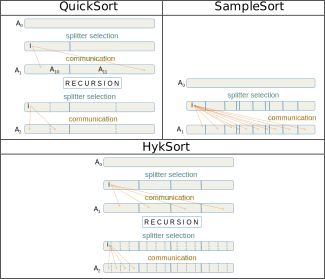
\includegraphics[width=0.7\linewidth]{ch_2/hyksort.pdf}}
    \caption{Communication pattern of Hyksort algorithm compared to a parallel Sample Sort, as well as a Quicksort over a hypercube, adapted from \cite{sundar2013hyksort}. We see that HykSort results in a lower communication overhead than Sample Sort.}
    \label{fig:sec_2_4:hyksort}
\end{figure}

\subsection*{Rusty Tree}

Developed using the algorithms described in the previous sections, Rusty Tree can be found at \url{https://github.com/rusty-fast-solvers/rusty-tree}. It is consumed either as a Rust crate or a Python package, with binaries distributed via Conda. We have so far tested Rusty Tree on MacOS as well as various Linux platforms including RHEL, common to many HPC platforms, and Ubuntu. With a fully developed suite of tests, documentation and Python interfaces, Rusty Tree represents a model example of our final software infrastructure for fast solvers. Example usage in Python mirrors the Rust interface as shown in listings (\ref{code:sec_2_4:rusty_py}) and (\ref{code:sec_2_4:rusty_rs}). Users are able use point data generated at runtime, or provide a HDF5 file for Rusty Tree to consume. Rusty Tree is also capable of outputting a VTK file for visualisation.  We follow data oriented principles in Rusty Tree's design, with a shallow abstraction layer that acts as an interface to operations on point data, and encoded Morton indices. An abridged software architecture in UML style is shown in figure (\ref{fig:sec_2_4:design}). In terms of lines of code, this translates into just 2578 lines of Rust and 688 lines of Python, including test code, with less than 100 lines of configuration code in terms of Toml and Yaml files specifying the Rust and Python builds.

The Python interfaces are built using Maturin, a tool for building and publishing Rust-based Python packages. It can do this in different ways, including the popular PyO3 \cite{pyo32022github} and rust-cpython \cite{rustcpython2022github} crates both of which offer Rust bindings for Python, allowing one to use Rust libraries as native extension modules as well as interacting with Python code from Rust binaries. However Maturin also supports creating bindings using Rust's C Foreign Function Interface (CFFI), using the \pythoninline{clib} crate to expose Rust types to consumers of the C application binary interface (ABI). We choose the CFFI, as the types we wish to expose into Rust are relatively simple pointers to Rust iterators and the pointer to an MPI communicator created from Python. This also allows for a simple design with minimal external libraries, with our Python interface to be cleanly separated from Rust source code.

\pythonexternal[basicstyle=\footnotesize, caption={Using Rusty Tree from its Python package.}\label{code:sec_2_4:rusty_py}]{snippets/rusty.py}

\rustexternal[basicstyle=\footnotesize, caption={Using Rusty Tree as a Rust library.}\label{code:sec_2_4:rusty_rs}]{snippets/rusty.rs}

\begin{figure}
    \centerline{
\includegraphics[width=\linewidth]{ch_2/rusty_tree_design.pdf}}
    \caption{We see that the shallow hierarchy inherent in Rusty Tree's design, with a `Distributed Tree' interface in both Python and Rust which is a wrapper over functionality that acts directly on data. On the Python side we have an additional \texttt{Iterator} class, that allows us to wrap Rust iterators into Python iterators.}
    \label{fig:sec_2_4:design}
\end{figure}

\subsubsection*{Using MPI from Rust}

MPI, via the rsMPI crate, constitutes the most complex dependency in Rusty Tree. The MPI bindings are built on top of C shim library, as well as automatically generated C/C++ compatible header files using the \pythoninline{cbindgen} crate. The shim library is used to form an equivalence between under-specified identifiers from the MPI standard, that may not be uniform across MPI implementations, and \pythoninline{cbindgen} is used to automatically generate headers for different MPI implementations. This allows rsMPI to expose an interface in Rust which covers most of MPI's core functionality for most MPI implementations, on most operating systems \footnote{This is an area of active development, and a list of currently supported features can be found here \url{https://github.com/rsmpi/rsmpi/blob/main/README.md}}. However, as it is designed to target multiple platforms like all other Rust crates, its build is fragile and requires extra configuration from users who might wish to deploy on unsupported or novel hardware and software targets. Specifically we have found to problems arise on Cray machines, such as Archer 2, which have custom installations of MPI and do not support the \texttt{mpicc} compiler wrapper. However, we note that this is an active area of development, and will be accounted for in a future rsMPI release. As a temporary fix, we currently fork of rsMPI with manual configurations to target the HPC systems we wish to run our software on. Consumers of our software will have to follow similar steps if automatic builds do not work, however we note that in the majority of cases this fragility will not be exposed to users, who can continue to who can continue to consume our library using a single line in their project's \pythoninline{Cargo.toml}. 

\subsection*{Scaling Experiments}

Figure (\ref{fig:sec_2_4:tree_comparison}a) shows the weak scaling performance of Rusty Tree\footnote{Experiments were taken on an AMD Ryzen Threadripper 3970X 32-Core processor} for constructing \textit{balanced octrees}. $5e5$ particles, taken from a random uniform distribution in a unit cube are placed on each processor, up to a total of 16 million particles. The parameter $n_crit$ is set to 200. We compare the performance of Rusty Tree with Dendro, a C++ library similarly built on algorithms presented in \cite{sundar2008bottom}. Dendro has a limited API in comparison to Rusty tree, with no Python interface, and no ability to query tree nodes for the points they contain and is therefore not usable for developing fast algorithms. However it does act as a showcase of the algorithms presented in \cite{sundar2008bottom}, allowing for a direct comparison to our own implementation. We observe that both softwares have a similar scaling behaviour for the tested problem sizes, however Rusty Tree is more expensive by a has a fixed constant factor, both in Python and Rust. We observe that this is due to our provision of hashmaps (see fig. (\ref{fig:sec_2_4:design})), that allow users to query tree nodes for the points they contain and vice versa, a functionality not available in Dendro. An experiment confirming this is shown in figure (\ref{fig:sec_2_4:tree_comparison}d).

We observe that Rusty Tree, when called from Python, has a significantly more expensive memory overhead in comparison to the Rust library, displayed in figure (\ref{fig:sec_2_4:tree_comparison}b). Whereas the Rust library, and Dendro, have similar memory profiles. The cause for excess memory overhead in Python is due to the need to assign static lifetimes to all Rust pointers passed to Python, for example for Morton keys and point data, which would be optimised out of a corresponding Rust program at compile time if it was not being used downstream in a program. We observe that the runtime cost of using Rusty Tree from Python is moderate, at between 5 and 25 \% of total runtime in Rust, for the problem sizes tested. 

Figure (\ref{fig:sec_2_4:tree_comparison}c) is a plot of the mean difference, of the load on each processor with respect to the mean load for a given geometry, as we scale a problem weakly. The geometries we choose are the surface of a `wiggly torus', as shown in figure (\ref{fig:octree_example:sec_1_2}), and the interior of a unit cube, where we sample $5e5$ points randomly from each domain at each processor. The parameter $n_{crit}$ is again set to 200. Comparing the results from both geometries, we observe a qualitatively weak dependence between the problem size and an increasing load imbalance. However, the overlapping nature of the error bars in our experiments, and the fact that an experiment with uniform random data shows similar load imbalance to a significantly less uniform data from the surface of a wiggly torus, make it difficult to conclude a correlation without further investigation. We will need to supplement this investigation with results for larger experiment sizes on large scale HPC systems.

\subsection*{Conclusion}

 Rusty Tree has high-level Python interfaces, allowing it to be inserted into existing research projects with minimal configuration with a moderate performance hit. It is designed around data and is simple to read, and importantly can be built for a variety of software and hardware environments. It's a demonstration of Rust as a viable alternative to development in Rust as opposed to C++ or Fortran. We believe that this will encourage the widespread adoption of our library, and we hope to publicise this software, as well as our user experience with Rust for high performance scientific computing, in an upcoming paper.

\begin{figure}
    \begin{tabular}{cc}
        \subfloat[\centering Runtime.]{\includegraphics[width=75mm]{ch_2/tree_weak_scaling.pdf}} & \subfloat[\centering Peak memory]{\includegraphics[width=75mm]{ch_2/tree_weak_scaling_mem.pdf}}
    \end{tabular}
    \begin{tabular}{cc}
    \centering \subfloat[\centering Load balancing]{\includegraphics[width=75mm]{ch_2/load_balance.pdf}} & \subfloat[\centering Runtime Breakdown]{\includegraphics[width=75mm]{ch_2/breakdown.pdf}}
    \end{tabular}
    \caption{There are $5e5$ points per processor for the weak scaling experiments in (a), with an $n_{crit}=200$.  Figure (b) shows the peak memory usage of Dendro compared to the Python and Rust interfaces of Rusty Tree. We note that the Python library has a significant overhead. Figure (c) shows the difference in load from the global mean load, as mean over runs, in an experiment that is weakly scaled with the same parameters as in figure (a). Figure (d) shows the breakdown in runtime between the different components of the algorithms for computing balanced and unbalanced trees, experiments are shown for a tree with $2e6$ uniformly randomly distributed points, distributed evenly across 4 processors. We see that the dominant factor in runtime is the creation of the hashmaps. }
    \label{fig:sec_2_4:tree_comparison}%
\end{figure}
